\documentclass[]{article}
\usepackage{lmodern}
\usepackage{amssymb,amsmath}
\usepackage{ifxetex,ifluatex}
\usepackage{fixltx2e} % provides \textsubscript
\ifnum 0\ifxetex 1\fi\ifluatex 1\fi=0 % if pdftex
  \usepackage[T1]{fontenc}
  \usepackage[utf8]{inputenc}
\else % if luatex or xelatex
  \ifxetex
    \usepackage{mathspec}
  \else
    \usepackage{fontspec}
  \fi
  \defaultfontfeatures{Ligatures=TeX,Scale=MatchLowercase}
\fi
% use upquote if available, for straight quotes in verbatim environments
\IfFileExists{upquote.sty}{\usepackage{upquote}}{}
% use microtype if available
\IfFileExists{microtype.sty}{%
\usepackage{microtype}
\UseMicrotypeSet[protrusion]{basicmath} % disable protrusion for tt fonts
}{}
\usepackage[margin=1in]{geometry}
\usepackage{hyperref}
\hypersetup{unicode=true,
            pdftitle={Project 1 - SPATIAL STATISTICS},
            pdfauthor={Kwaku Peprah Adjei, Amir Ahmed},
            pdfborder={0 0 0},
            breaklinks=true}
\urlstyle{same}  % don't use monospace font for urls
\usepackage{color}
\usepackage{fancyvrb}
\newcommand{\VerbBar}{|}
\newcommand{\VERB}{\Verb[commandchars=\\\{\}]}
\DefineVerbatimEnvironment{Highlighting}{Verbatim}{commandchars=\\\{\}}
% Add ',fontsize=\small' for more characters per line
\usepackage{framed}
\definecolor{shadecolor}{RGB}{248,248,248}
\newenvironment{Shaded}{\begin{snugshade}}{\end{snugshade}}
\newcommand{\AlertTok}[1]{\textcolor[rgb]{0.94,0.16,0.16}{#1}}
\newcommand{\AnnotationTok}[1]{\textcolor[rgb]{0.56,0.35,0.01}{\textbf{\textit{#1}}}}
\newcommand{\AttributeTok}[1]{\textcolor[rgb]{0.77,0.63,0.00}{#1}}
\newcommand{\BaseNTok}[1]{\textcolor[rgb]{0.00,0.00,0.81}{#1}}
\newcommand{\BuiltInTok}[1]{#1}
\newcommand{\CharTok}[1]{\textcolor[rgb]{0.31,0.60,0.02}{#1}}
\newcommand{\CommentTok}[1]{\textcolor[rgb]{0.56,0.35,0.01}{\textit{#1}}}
\newcommand{\CommentVarTok}[1]{\textcolor[rgb]{0.56,0.35,0.01}{\textbf{\textit{#1}}}}
\newcommand{\ConstantTok}[1]{\textcolor[rgb]{0.00,0.00,0.00}{#1}}
\newcommand{\ControlFlowTok}[1]{\textcolor[rgb]{0.13,0.29,0.53}{\textbf{#1}}}
\newcommand{\DataTypeTok}[1]{\textcolor[rgb]{0.13,0.29,0.53}{#1}}
\newcommand{\DecValTok}[1]{\textcolor[rgb]{0.00,0.00,0.81}{#1}}
\newcommand{\DocumentationTok}[1]{\textcolor[rgb]{0.56,0.35,0.01}{\textbf{\textit{#1}}}}
\newcommand{\ErrorTok}[1]{\textcolor[rgb]{0.64,0.00,0.00}{\textbf{#1}}}
\newcommand{\ExtensionTok}[1]{#1}
\newcommand{\FloatTok}[1]{\textcolor[rgb]{0.00,0.00,0.81}{#1}}
\newcommand{\FunctionTok}[1]{\textcolor[rgb]{0.00,0.00,0.00}{#1}}
\newcommand{\ImportTok}[1]{#1}
\newcommand{\InformationTok}[1]{\textcolor[rgb]{0.56,0.35,0.01}{\textbf{\textit{#1}}}}
\newcommand{\KeywordTok}[1]{\textcolor[rgb]{0.13,0.29,0.53}{\textbf{#1}}}
\newcommand{\NormalTok}[1]{#1}
\newcommand{\OperatorTok}[1]{\textcolor[rgb]{0.81,0.36,0.00}{\textbf{#1}}}
\newcommand{\OtherTok}[1]{\textcolor[rgb]{0.56,0.35,0.01}{#1}}
\newcommand{\PreprocessorTok}[1]{\textcolor[rgb]{0.56,0.35,0.01}{\textit{#1}}}
\newcommand{\RegionMarkerTok}[1]{#1}
\newcommand{\SpecialCharTok}[1]{\textcolor[rgb]{0.00,0.00,0.00}{#1}}
\newcommand{\SpecialStringTok}[1]{\textcolor[rgb]{0.31,0.60,0.02}{#1}}
\newcommand{\StringTok}[1]{\textcolor[rgb]{0.31,0.60,0.02}{#1}}
\newcommand{\VariableTok}[1]{\textcolor[rgb]{0.00,0.00,0.00}{#1}}
\newcommand{\VerbatimStringTok}[1]{\textcolor[rgb]{0.31,0.60,0.02}{#1}}
\newcommand{\WarningTok}[1]{\textcolor[rgb]{0.56,0.35,0.01}{\textbf{\textit{#1}}}}
\usepackage{longtable,booktabs}
\usepackage{graphicx,grffile}
\makeatletter
\def\maxwidth{\ifdim\Gin@nat@width>\linewidth\linewidth\else\Gin@nat@width\fi}
\def\maxheight{\ifdim\Gin@nat@height>\textheight\textheight\else\Gin@nat@height\fi}
\makeatother
% Scale images if necessary, so that they will not overflow the page
% margins by default, and it is still possible to overwrite the defaults
% using explicit options in \includegraphics[width, height, ...]{}
\setkeys{Gin}{width=\maxwidth,height=\maxheight,keepaspectratio}
\IfFileExists{parskip.sty}{%
\usepackage{parskip}
}{% else
\setlength{\parindent}{0pt}
\setlength{\parskip}{6pt plus 2pt minus 1pt}
}
\setlength{\emergencystretch}{3em}  % prevent overfull lines
\providecommand{\tightlist}{%
  \setlength{\itemsep}{0pt}\setlength{\parskip}{0pt}}
\setcounter{secnumdepth}{0}
% Redefines (sub)paragraphs to behave more like sections
\ifx\paragraph\undefined\else
\let\oldparagraph\paragraph
\renewcommand{\paragraph}[1]{\oldparagraph{#1}\mbox{}}
\fi
\ifx\subparagraph\undefined\else
\let\oldsubparagraph\subparagraph
\renewcommand{\subparagraph}[1]{\oldsubparagraph{#1}\mbox{}}
\fi

%%% Use protect on footnotes to avoid problems with footnotes in titles
\let\rmarkdownfootnote\footnote%
\def\footnote{\protect\rmarkdownfootnote}

%%% Change title format to be more compact
\usepackage{titling}

% Create subtitle command for use in maketitle
\providecommand{\subtitle}[1]{
  \posttitle{
    \begin{center}\large#1\end{center}
    }
}

\setlength{\droptitle}{-2em}

  \title{Project 1 - SPATIAL STATISTICS}
    \pretitle{\vspace{\droptitle}\centering\huge}
  \posttitle{\par}
    \author{Kwaku Peprah Adjei, Amir Ahmed}
    \preauthor{\centering\large\emph}
  \postauthor{\par}
    \date{}
    \predate{}\postdate{}
  
\usepackage[utf8]{inputenc}
\usepackage{amsmath}
\usepackage{amssymb}
\usepackage{graphicx}
\usepackage{caption}
\usepackage{subcaption}
\graphicspath{ {./images/} }

%vector: 
\newcommand{\vect}[1]{\ensuremath{\boldsymbol{\mathbf{#1}}}} 
%matrix: 
\newcommand{\matr}[1]{\ensuremath{\boldsymbol{\mathbf{#1}}}}

\DeclareMathOperator{\Cov}{\text{Cov}}

\DeclareMathOperator{\iid}{\text{iid}}

\begin{document}
\maketitle

\newpage

\hypertarget{problem-1}{%
\section{Problem 1}\label{problem-1}}

Let
\(\lbrace r(x) : x \in \text{D} : \left[1, 50\right]\subset\mathbb{R}^1\rbrace\).
Assume it is modelled as a stationary one dimensional Gaussian random
field with the following parameters: \begin{equation}\label{prob1eq}
    \begin{split}
    E\lbrace r(x) \rbrace &= \mu_r = 0 \\
    Var\lbrace r(x)\rbrace &= \sigma_r^2 \\
    Corr\lbrace r(x), r(x')\rbrace &= \rho_r(\tau) \\
    \tau = \dfrac{|x-x'|}{10}
    \end{split}
\end{equation} where \(\rho_r(\tau)\) is the spatial correlation
function. Discretize \(D\) as \(L = \lbrace 1, 2, \dots, 50 \rbrace\),
we will later look at the discretized Gaussian random field
\(\lbrace r(x) : x\in L \rbrace\).

\hypertarget{problem-1a}{%
\subsection{Problem 1a}\label{problem-1a}}

To ensure the positive definetness of all covariance matrices, we rely
on having a positve definite corrolation function. A positive definite
correlation function guarantees that the covariance matrix of our
Gaussian random field is well defined for all choices of observation
points and for all dimensions.

A function \(c(\vect \tau): \mathbb{R}^q\) i positive definite if the
following is satisfied: \begin{equation}\label{posdefeq}
    \begin{split}
        \sum_{i=1}^n\sum_{j=1}^n\alpha_i\alpha_j c(\vect x_i - \vect x_j) \geq 0,
    \end{split}
    \quad
    \begin{split}
        &\forall \alpha_1, \dots, \alpha_n \in \mathbb{R} \\
        &\forall n \in \mathbb{N}, \quad n \geq 2 \\
        &\forall \vect x_1, \dots \vect x_n \in \mathbb{R}^q
  \end{split}
\end{equation} Any \(n \times n\) matrix,
\(\matr Q = \left[ c(\vect x_i - \vect x_j) \right]_{ij}\) constructed
with a positive definite \(c(\vect \tau)\) with vectors
\(\lbrace \vect x_i \rbrace_{i=1}^n\) chosen as in \eqref{posdefeq}
would clearly be positive definite. As for all
\(\vect \alpha = (\alpha_1, \dots, \alpha_n) \in \mathbb{R}^n\) we have:
\begin{equation}
    \vect \alpha^T \matr Q \vect \alpha =   \sum_{i=1}^n\sum_{j=1}^n\alpha_i\alpha_j c(\vect x_i - \vect x_j) \geq 0
\end{equation} So it would be safe to use \(\matr Q\) as a covariance
matrix, and it would satisfy the requirements of the multivariate normal
distribution.

We now go on to look at the the powered exponential correlation
function:

\begin{equation}
    \begin{split}
            \rho(\tau) = \exp(-\tau^{\nu}) 
    \end{split}, \quad
    \begin{split}
    \nu \in \left(0, 2 \right]
    \end{split}
\end{equation} for later case studies we will look at parameters
\(\nu_r \in \lbrace 1, 1.9 \rbrace\). We note that and increased \(\nu\)
(\(\nu >> 1\)) would lower the exponent and thus give less correlation.

We also want to study the Matern correlation function \begin{equation}
    \begin{split}
            \rho_r(\tau) = \dfrac{2^{1-\nu}}{\Gamma(\nu)}\tau^v\mathcal{B}_\nu(\tau), \quad
    \end{split}
    \begin{split}
        \nu \in \mathbb{R}_+
    \end{split}
\end{equation} \(\mathcal{B}_\nu\) is the bessel function. We want to
look at the matern with parameters \(\nu_r \in \lbrace 1, 3 \rbrace\).

For both correlation functions use
\(\sigma^2_r \in \lbrace 1, 5\rbrace\)

\begin{figure}
\centering
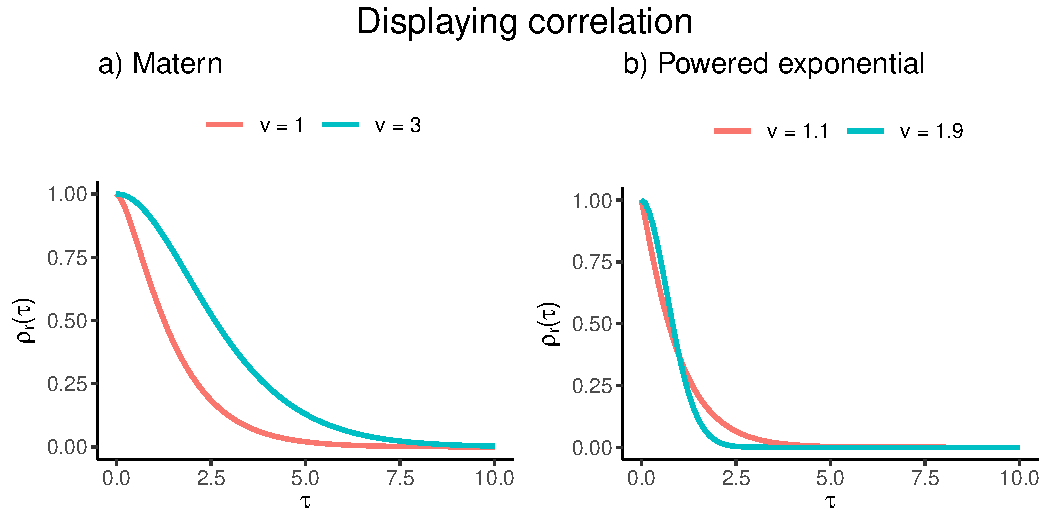
\includegraphics{Exercise-1_files/figure-latex/fig1a1-1.pdf}
\caption{\label{fig:fig1a1} Plotting matern and exponential correlation}
\end{figure}

The two correlation functions are plotted in Figure \ref{fig:fig1a1} for
\(\tau \in \mathbb{R}_\oplus\). We note that these functions both are
positive definite. From the figures we also note that both correlation
functions for the different parameters seems to satisfy ergodicity,
correlation drops to zero the further apart to points are, this is a
neccesary trait in our Gaussian RF.

For the matern corrolation we see that an increase of \(\nu\) lead to
slower fall in correlation with distance. We also note that the Matern
seems to drop slower in correlation than the exponential correlation
function for the given parameters.

For higher values of \(\nu\) and when \(\tau >> 1\) the powered
exponential seems to drop faster in correlation than for higher \(\nu\).
The oppsite seems to be the trend when \(\tau << 1\)

The variogram function is defined as:
\begin{equation}\label{eq:variogram}
    \begin{split}
        \gamma_r(\tau)  &= \frac{1}{2} Var\lbrace r(x) - r(x') \rbrace \\
        &= \frac{1}{2} (Var\lbrace r(x) \rbrace + Var\lbrace r(x') \rbrace - 2 Corr\lbrace r(x), r(x')) \rbrace\\
        &=\sigma_r^2(1-\rho_r(\tau))
    \end{split}
\end{equation}

Looking at \eqref{eq:variogram} we see that if \(\sigma_r^2 = 1\) then
the corrolation function and the variogram functions would respectively
increase and decrease at same rate in with respect to an increase in
\(\tau\). In essence the variogram function tells us how much variance
we have in our estimation of \(x'\) when it is \(\tau\) away from a
observed point \(x\)

\begin{figure}
\centering
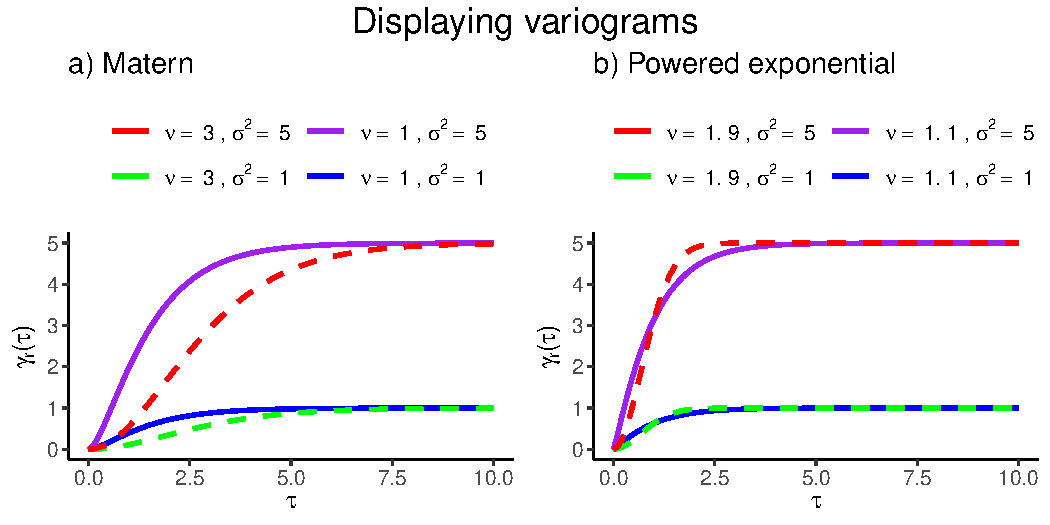
\includegraphics{Exercise-1_files/figure-latex/fig1a2-1.pdf}
\caption{\label{fig:fig1a2} Plotting variograms}
\end{figure}

We display the variograms for our model parameters in Figure
\ref{fig:fig1a2}.

In both figures we see that the value of \(\sigma^2\) sets a roof on the
variance of points far away. Higher values of \(\sigma^2\) also seems to
increase the max achieved variance. For the matern variogram increased
\(\nu\) seems to increase corrolation to neighbouring points.

\newpage

\hypertarget{problem-1b}{%
\subsection{Problem 1b}\label{problem-1b}}

We use the corrolation function \(\rho_r(\tau)\) to construct a
corrolation matrix. The corrolation matrix would have the following
form: \begin{equation}
    \matr \Sigma_r^\rho = 
    \begin{bmatrix}
        \rho_r(1, 1) & \rho_r(1, 2) & \dots & \rho_r(1, 50) \\
        \rho_r(2, 1) & \rho_r(2, 2) & \dots & \rho_r(2, 50) \\
        \vdots & \vdots & \ddots & \vdots \\
        \rho_r(50, 1) & \rho_r(50, 2) & \dots & \rho_r(50, 50)
    \end{bmatrix}
\end{equation} \(\rho_r(x, x')\) denotes
\(\rho_r(\tau) = \rho_r(|x-x'|/10)\). With variance \(\sigma_r^2\) the
prior get the covariance matrix
\(\matr \Sigma_r = \sigma_r^2 \matr \Sigma_r^\rho\). From
\eqref{prob1eq} we have an expected value of: \begin{equation}
    \vect \mu_r = (0, \dots, 0)^T
\end{equation} Which gives the prior a distribution of: \begin{equation}
    \phi_{50}(\vect r ; \vect \mu_r, \matr \Sigma_r)
\end{equation} Which has pdf: \begin{equation}
    (2\pi)^{-\frac{50}{2}}\det(\matr \Sigma_r)^{-\frac{1}{2}}\exp\left(-\frac{1}{2}\vect x^T\matr \Sigma_r^{-1}\vect x\right)
\end{equation}

We simulate four realisations of the field for the different parameters.

\begin{figure}

{\centering 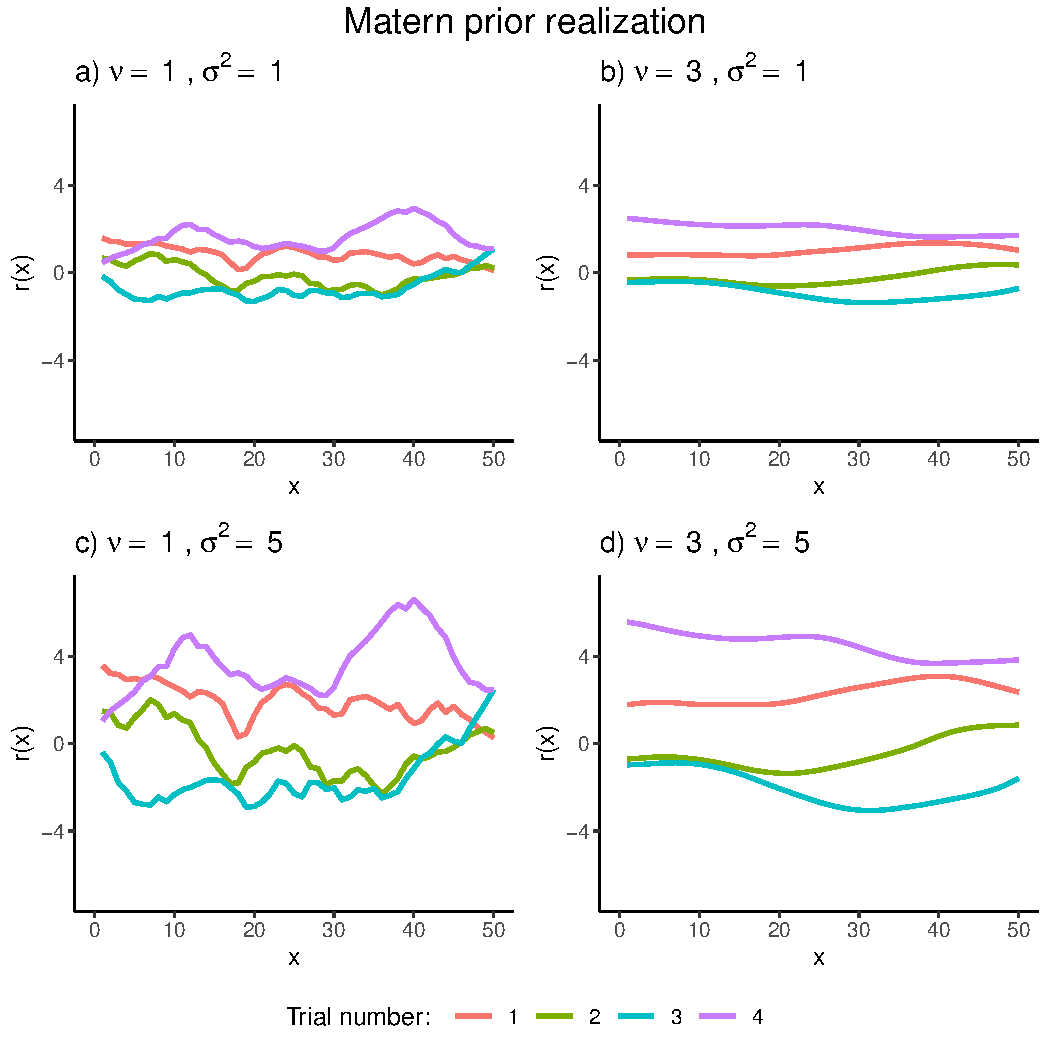
\includegraphics{Exercise-1_files/figure-latex/fig1b1-1} 

}

\caption{\label{fig:fig1b1} Realizisations of prior, matern}\label{fig:fig1b1}
\end{figure}

\begin{figure}

{\centering 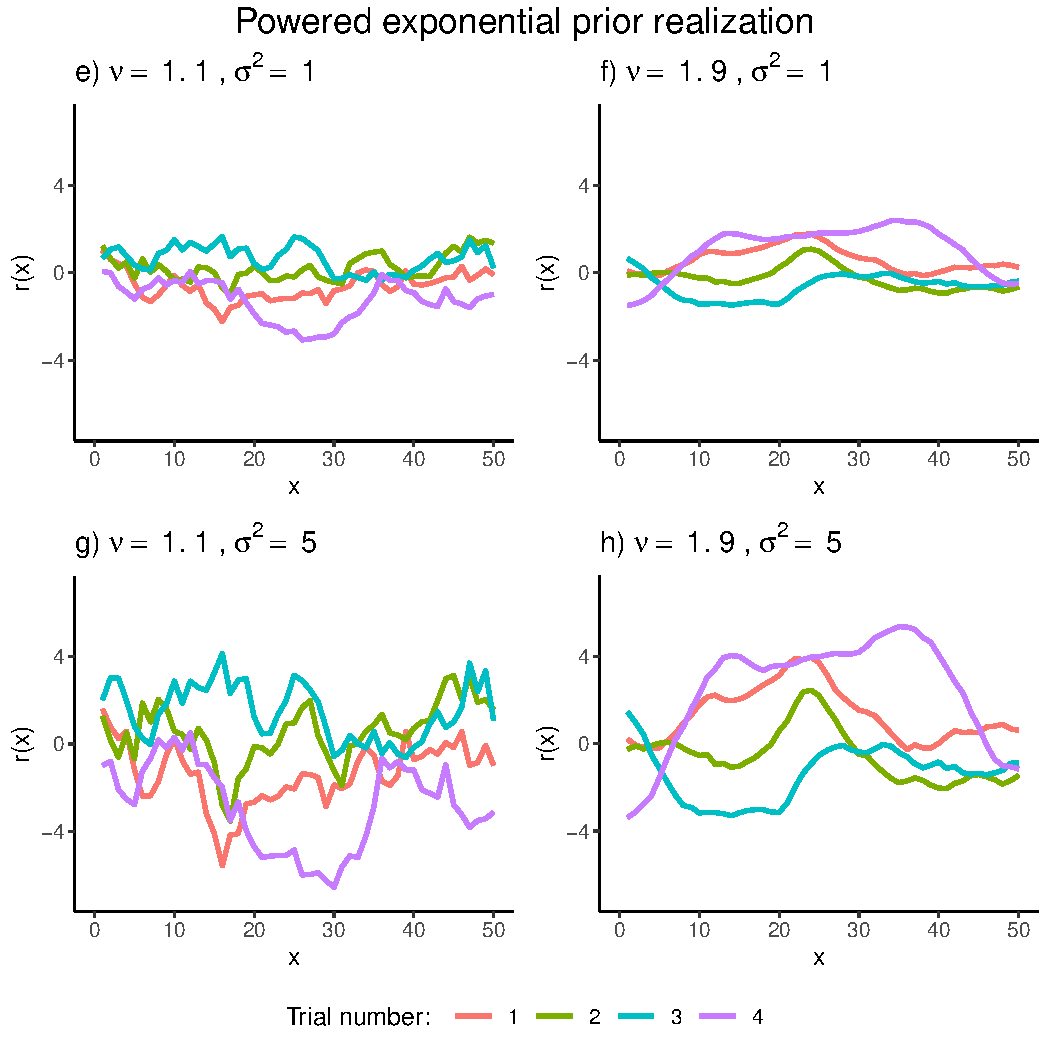
\includegraphics{Exercise-1_files/figure-latex/fig1b2-1} 

}

\caption{\label{fig:fig1b2} Realizisations of prior, powered exponential}\label{fig:fig1b2}
\end{figure}

The results are plotted in Figure \ref{fig:fig1b1} and Figure
\ref{fig:fig1b2}. We note that an increased variance seems to increase
fluctuation (comparing c) d) g) and h) to the others). For the matern we
also see that an increased \(\nu\) seems to make the process smoother.
For both correlation functions increased \(\nu\) seems to increase
``air-time'' when the process is strays away from expected 0.

\newpage

\hypertarget{problem-1c}{%
\subsection{Problem 1c}\label{problem-1c}}

We now want to develop a posterior model. Assume that we have observed
the values at \(x \in \lbrace 10, 25, 30 \rbrace\). Organise them as:
\begin{equation}
    \lbrace d(x); x \in \lbrace 10, 25, 30 \rbrace \subset L  \rbrace 
\end{equation} We also assume we have an observation error
\(\sigma^2_\epsilon = \lbrace 0, 0.25 \rbrace\). In general we have
\begin{gather}
    d(x) = r(x) + \epsilon(x), \quad x \in \lbrace 10, 25, 30 \rbrace \\
   \epsilon(x) \sim N(0, \sigma_\epsilon^2), \iid \\
   r(x) \text{ and } \epsilon(x) \text{ independent} \\
   \epsilon(x) \text{ and } \epsilon(x') \text{ independent identically distributed} 
\end{gather}

As \(\epsilon(x)\) and \(r(x)\) are Gaussian, a linear product of the
two would also be.

We further note: \begin{equation}
    E(d(x)) = E(r(x)) + E((\epsilon(x))) = 0
\end{equation} When \(x\neq x'\) \begin{equation*}
    \begin{split}
        \Cov(d(x), d(x')) &= \Cov(r(x)+\epsilon(x), r(x') + \epsilon(x')) \\
        &= \Cov(r(x), r(x')) + \Cov(\epsilon(x), \epsilon(x')) \\
        &= \sigma_r^2\rho_r(\tau)
    \end{split}
\end{equation*} otherwise: \begin{equation}
    \begin{split}
        \Cov(d(x), d(x)) &= \Cov(r(x)+\epsilon(x), r(x) + \epsilon(x)) \\ 
        &= \Cov(r(x), r(x)) + \Cov(\epsilon(x), \epsilon(x)) \\
        &= \sigma_r^2\rho_r(\tau) + \sigma_e^2
    \end{split}
\end{equation} We organise the observed points in a \(k \times 1\)
vector,\(\vect y = (10, 25, 30)^T\), where \(k = 3\). Further let the
observed values of the random field be: \begin{equation}
    \vect d(\vect y) = ( d(10), d(25), d(30))^T
\end{equation} If we denote \(\matr \Sigma_\rho^d\) as the correlation
matrix generated by \(\rho(\tau)\) between the points \(\vect x\) we
see: \begin{equation}
    \Cov(\vect d(\vect x), \vect d(\vect x')) = \sigma^2_e \matr I_k +\sigma^2_r\matr \Sigma^\rho_d
\end{equation}

Using the calculations above \(\vect d\) thus have the following pdf:
\begin{equation}
    p(\vect d(\vect x)|\sigma_r^2, \sigma_e^2) = (2\pi)^{k/2}\det(\matr \Sigma_\rho^d)^{-1/2}\exp(\frac{1}{2}\vect d^T(\matr\Sigma_\rho^d)^{-1}\vect d)
\end{equation} The value \(\sigma_e^2\) would then have the following
likelihood function: \begin{equation}
    L(\sigma_e^2 | \vect d(\vect x), \sigma_r^2)=p(\vect d(\vect x)|\sigma_r^2, \sigma_e^2)
\end{equation} The integral \begin{equation}
    \int_{0}^{\infty}L(\sigma_e^2 | \vect d(\vect x), \sigma_r^2)d\sigma^2
\end{equation} goes to infinity, thus
\(L(\sigma_e^2 | \vect d(\vect x), \sigma_r^2)\) is not a pdf. If we try
to estimate \(\sigma^2_\epsilon\) by the expected value of
\(\sigma_e^2\) derived when believing \(L(\sigma^2_\epsilon|\cdot)\) is
a pdf, we would expect values that goes to infinity, which would be
wrong.

\hypertarget{problem-1d}{%
\subsection{Problem 1d}\label{problem-1d}}

Assume now that \(\sigma_r^2 = 5\) and that we have observed
\(\vect d(\vect y)\) with error
\(\sigma_\epsilon^2 = \in \lbrace 0, 0.25 \rbrace\). Want to find the
distribution of \(\left[ \vect r | \vect d \right]\). Know that both
\(\vect r\) and \(\vect d\) are multivariate normal. Thus conditioning
\(\vect r\) on \(\vect d\) would give a multivariate normal distribution
with the following parameters:

\begin{equation}
     \vect\mu_{\vect r | \vect d} = \vect \mu_r+ \matr \Sigma_{\vect r, \vect d} \matr \Sigma_{\vect d}^{-1}(\vect d - \vect \mu_{\vect d})
\end{equation}

\begin{equation}
      \vect\Sigma_{\vect r | \vect d} = \matr \Sigma_{\vect r} - \matr \Sigma_{\vect r, \vect d} \matr \Sigma_{\vect d}^{-1}\Sigma_{\vect d, \vect r}
\end{equation}

Note \(\Sigma_{\vect r, \vect d} = \Sigma_{\vect d, \vect r}^T\) and
they are respectively \(50\times 3\) and \(3\times 50\) where the first
has elements \([\Cov\lbrace r(x_i), d(x_j)\rbrace]_{ij}\) where:

\begin{equation}
    \begin{split}
        \Cov\lbrace r(x_i), d(x_j)\rbrace &= \Cov\lbrace r(x_i), r(x_j) + \epsilon(x_j)\rbrace  \\
        &= \Cov\lbrace r(x_i), r(x_j)\rbrace \\ 
        &= \sigma_r^2\rho_r(x_i, x_j)
    \end{split}
\end{equation}

Assuming we have realisations of \(\vect d\) from simulated data we can
study how \(\vect r | \vect d\) acts.

\begin{figure}

{\centering 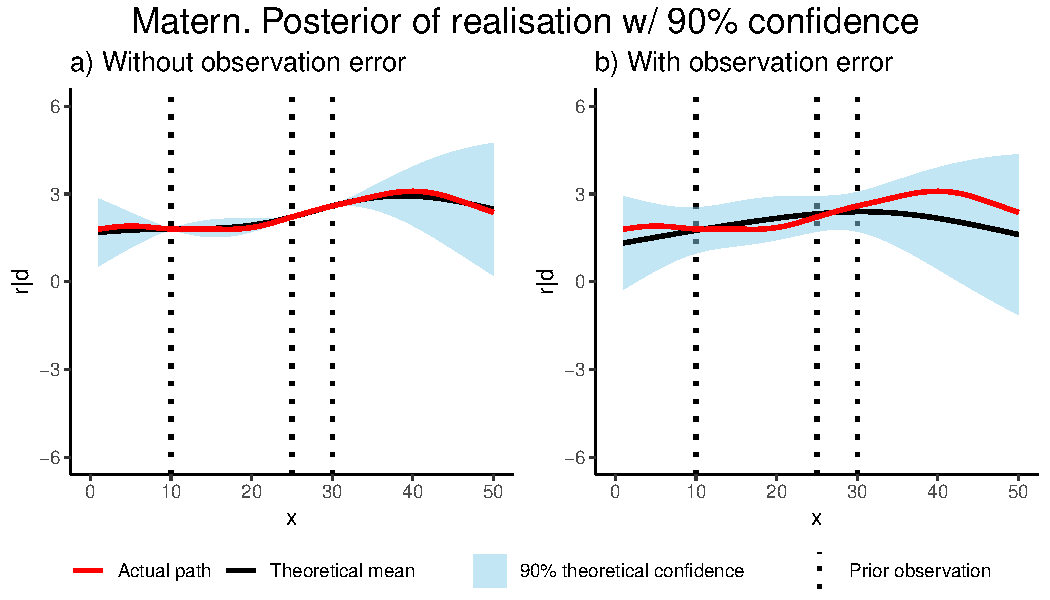
\includegraphics{Exercise-1_files/figure-latex/fig1d1-1} 

}

\caption{\label{fig:fig1d1} Posterior estimation, matern $\sigma^2 = 5$, $\nu = 3$}\label{fig:fig1d1}
\end{figure}

We compute two corresponding predictions for the spatial variable
\(\lbrace \hat r(x);x \in L\rbrace\) with associated 0.9 predictions
intervals and display them in Figure \ref{fig:fig1d1}. We use the same
realisations Trial 1 in d) in Figure \ref{fig:fig1b1}.

Here we have parameters \(\nu_r = 3\) and \(\sigma_r^2 = 5\). As
discussed earlier, we would with these values see much corrolation. From
the variogram, points with distance up to about 20 in distance would
impact each other, this is reflected in the figure, as the observation
points shifts large parts of the process away from 0. The high
correlation decreases the width of the 90\% confidence intervals close
to the observations. In the interval \(x\in (25,30)\) the 90\% band is
very narrow in the exact observation case, comapred to the one with
observation error. Comparing no variance in observation to variance the
points close to the observation points in no observation error is of
course more accurate, but further away i.e.~at point 20 the increased
variance seem to have little impact on the confidence band. The real
process behind, keeps within 90\% although we would expect more of them
to stray of, as we have 47 non observed-points.

\hypertarget{problem-1e}{%
\subsection{Problem 1e}\label{problem-1e}}

We now simulate 100 realisation's with the same parameters as in 1d) and
calculate empirical mean and empirical 90\% confidence bands.

\begin{figure}

{\centering 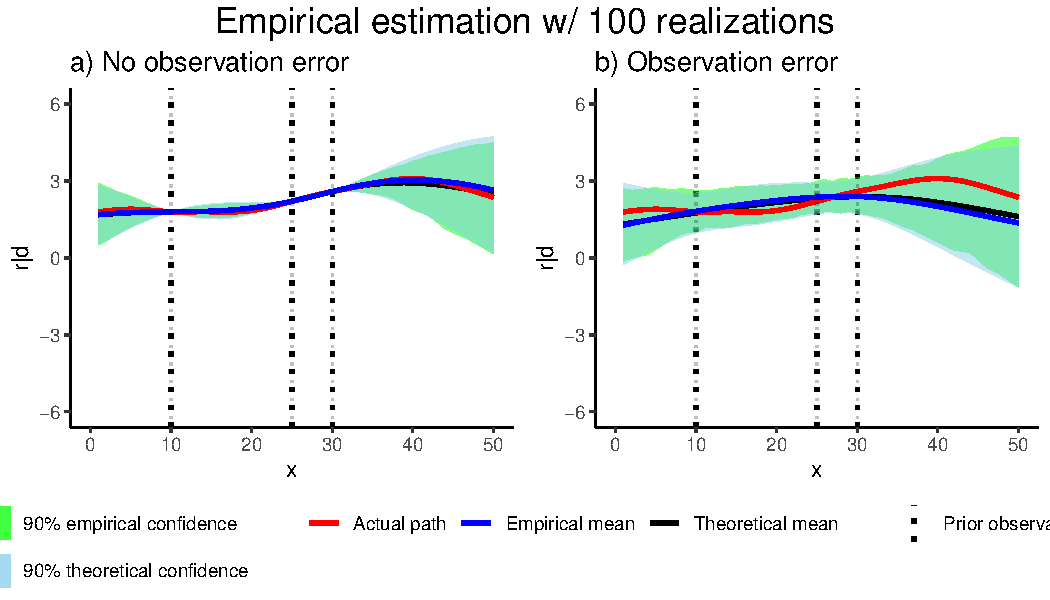
\includegraphics{Exercise-1_files/figure-latex/fig1e1-1} 

}

\caption{\label{fig:fig1e2} Posterior estimation 100 realisation, matern $\sigma^2 = 5$, $\nu = 3$}\label{fig:fig1e1}
\end{figure}

The results are illustrated in Figure \ref{fig:fig1e2}. We also include
the theoretical plots that the simulations are drawn from. For both with
observation error and without observations error the empirical
estimations seems to do well, and overlaps quite well with the
theoretical bands. The largest differences between the two are seen
furthest away from the observations points. Between \(x\in(10,25)\)
theoretical bands seems to have a slight tendency to be wider that the
empirical bands, however the trend is not too clear. Close to the
observation points the bands seems to be equally wide without
observation error, with obserbation error there seems to be slightly
more variation.

\hypertarget{problem-1f}{%
\subsection{Problem 1f}\label{problem-1f}}

Want to evaluate

\begin{equation}
    A_r = \int_D I(r(x) > 2)(r(x)-2) dx
\end{equation}

\begin{figure}

{\centering 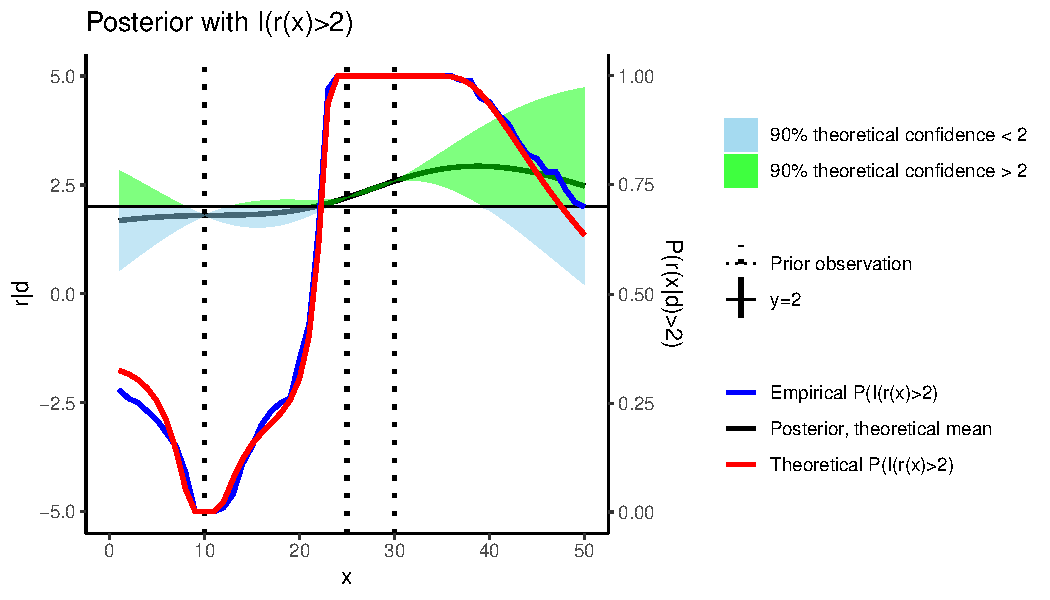
\includegraphics{Exercise-1_files/figure-latex/fig1f1-1} 

}

\caption{\label{fig:fig1f1} Posterior estimation 100 realisation, matern $\sigma^2 = 5$, $\nu = 3$}\label{fig:fig1f1}
\end{figure}

The situation with \(I(r(x)>2)\) is displayed in Figure
\ref{fig:fig1f1}.

A prediction of the integral using our 100 realizations from the
posterior model with \(\sigma_\epsilon^2\) is:

\begin{equation}
    \hat{A}_r = \frac{1}{100}\sum_{i=1}^{100}\sum_{x\in L}I(r_i(x)>2)(r(x)-2)
\end{equation}

Applying this to our realisation we get: \(\hat A_r =\) 22.9350097 and
\(Var(\hat A) =\) 104.8484493

Another estimator is: \begin{equation}
    \tilde A_r = \sum_{x \in L} I(\hat r(x) > 2)(\hat r(x) - 2)
\end{equation} With our data we get: \(\tilde A_r =\) 18.3398699

If we let: \begin{equation}
    g(r(x)) = \int_D I(r(x) > 2)(r(x) - 2) dx
\end{equation} Then \(g(x)\) is convex as it is an integral of a
positive value.

Using Jensen's Inequality we thus get: \begin{equation}
 Eg(r(x)) \geq g(Er(x)) = \int_D I(Er(x) > 2)(Er(x) - 2) = \tilde A_r
\end{equation} The same would be the case for the discretized stimators,
i.e.~we have: \[E\hat A_r \geq \tilde A_r\] And is why we expect
\(\hat A_r > \tilde A_r\). Which is also what we observed.

\hypertarget{problem-1g}{%
\section{Problem 1g)}\label{problem-1g}}

We have studied the matern and the powered exponential correlation
function, and applied them to simulated data, to estiamte posteriors and
their confidence. We find it interesteing how a change in the \(\nu\)
seem to change the differentiability of the end smoothness. Overall the
empirical estimation methods seems to work well and are consistent with
theory.

\newpage

\hypertarget{problem-2-gaussian-rf---real-data}{%
\section{Problem 2 Gaussian RF - real
data}\label{problem-2-gaussian-rf---real-data}}

Given the domain \(D = [(0,315) \times (0,315)] \subset \mathbb{R^2}\).
We let \(\vect{d}= r(\vect{x_1^0)}, ..., r(\vect{x_{52}^0)})^T\).

\hypertarget{problem-2a-display-of-the-data}{%
\subsection{Problem 2a: Display of the
data}\label{problem-2a-display-of-the-data}}

The data is displayed with an image plot, a contour plot and the exact
points as shown in the figure \ref{fig:fig1} below.
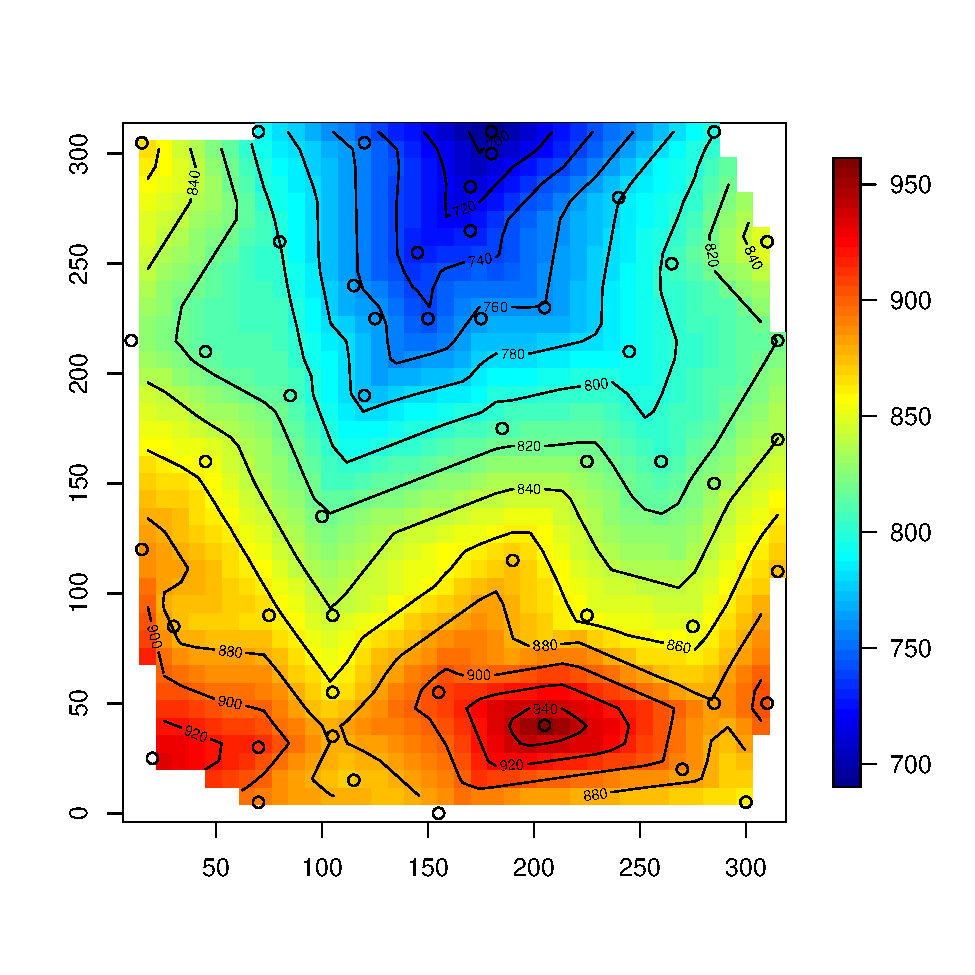
\includegraphics{Exercise-1_files/figure-latex/fig1-1.pdf}

It was observed that the data points did not move in the same direction
as with the x and y cordinates (see figure \ref{fig:fig2} a;b). This
suggest that the data is not mean stationary. Moreover, a density plot
for the data points in figure \ref{fig:fig2} c) shows a skewness in the
data, making the Guassianity assumption doubtful. Hence a stationary
Gaussian RF may not be appropriate.

\begin{figure}
\centering
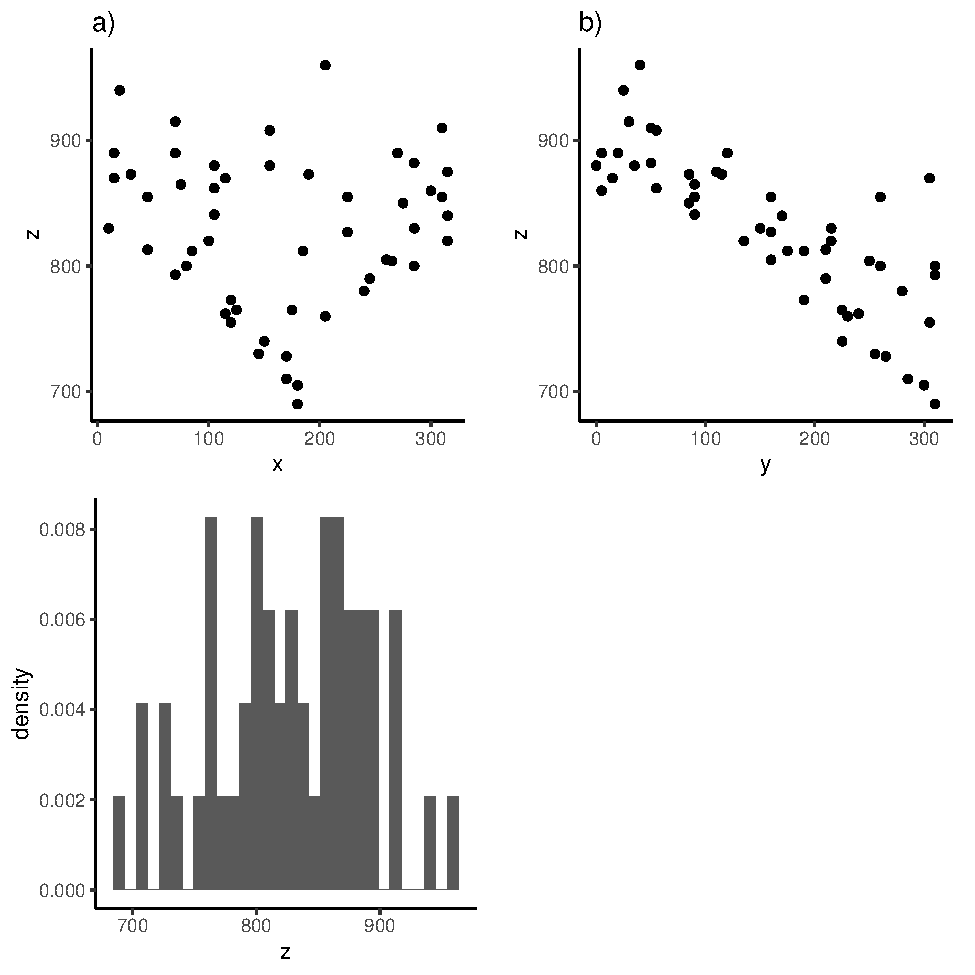
\includegraphics{Exercise-1_files/figure-latex/fig2-1.pdf}
\caption{\label{fig:fig2} Plot of the data points with respect to their
a) x-cordinates and b) y-cordinates; and c) shows the density
distribution of the terrain elevation observations.}
\end{figure}

\hypertarget{problem-2b}{%
\subsection{Problem 2b}\label{problem-2b}}

Let \[
\{r (\vect{x}); \vect{x} \in D \subset \mathbb{R^2}\}
\] be the Gaussian RF that is used to model the domain \(D\).

Given that \(E\{r(x)\} = (\vect{gx})^T \vect{\beta_r}\),
\(Var\{r(\vect{x})\} = \sigma_r^2\) and
\(Corr(r(\vect{x}), r(\vect{x'})) = \rho_r(\frac{\tau}{\xi})\). We
assume that \(\sigma_r^2, \xi\) are assumed known but \(\vect{\beta_r}\)
is unknown. This is therefore a universal krigging problem.

Let the krigging predictor be: \[
\vect{\hat{r}_0} = \vect{\alpha}^T \vect{r^d} 
\]

We discretise the predictor as: \[
\{\vect{r_{\Delta} (x)} = r(\vect{x}) - \mu_r^0 - \sum_{i=1}^{n_g} \beta_r^j g_j(\vect{x}); \vect{x} \in  D\}
\]

For the estimator to be unbiased,

\[E\{\vect{\hat{r}_0} - \vect{{r}_0} =0 \} \implies \sum_{i=1}^m \alpha_iE\{r_i^d\} - E\{ \vect{{r}_0}\} = 0\]

\[\sum_{i=1}^m \sum_{j=1}^{n_g} \alpha_i \beta_r^j g_j(\vect{x}_i) = \sum_{j}\beta_r^j g_j(\vect{x}_0)\]

For the estimator to be unbiased,

\(\sum_{i=1}^m \alpha_i g_j(\vect{x}_i) = \sum_{j}\beta_r^j g_j(\vect{x}_0)\).

\begin{equation*}
    \begin{split}
      Var\{\vect{\hat{r}_0} - \vect{{r}_0} \} &= E\{(\vect{\hat{r}_0} - \vect{{r}_0})^2 \} \\
                                       &= Var\{\alpha_i \{r_i^d\} - \vect{{r}_0}\} \\
                                        &= \sigma^2 \sum_{i=1}^n\sum_{j=1}^m \alpha_i\alpha_j\rho_{ij} + \sigma^2 + 2 \sigma^2\sum_{j=1}^m\alpha_j\rho_{j0}\\
    \end{split}
\end{equation*}

Hence, we find \(\vect{\hat\alpha}\) such that \[
\vect{\hat\alpha} = argmin_{\vect{\alpha}} Var\{\vect{\hat{r}_0} - \vect{{r}_0} \}
\] and subject to the constraint
\(\sum_{i=1}^m \alpha_i g_j(\vect{x}_i) = \sum_{j}\beta_r^j g_j(\vect{x}_0)\)
for \(j= 1,2,...,n_g\).

\hypertarget{problem-2c}{%
\subsection{Problem 2c}\label{problem-2c}}

Considering the case with \(E(r(\vect x)) = \beta_1\), we estimated the
universal krigging predictor and variance as follows:

\begin{figure}
\centering
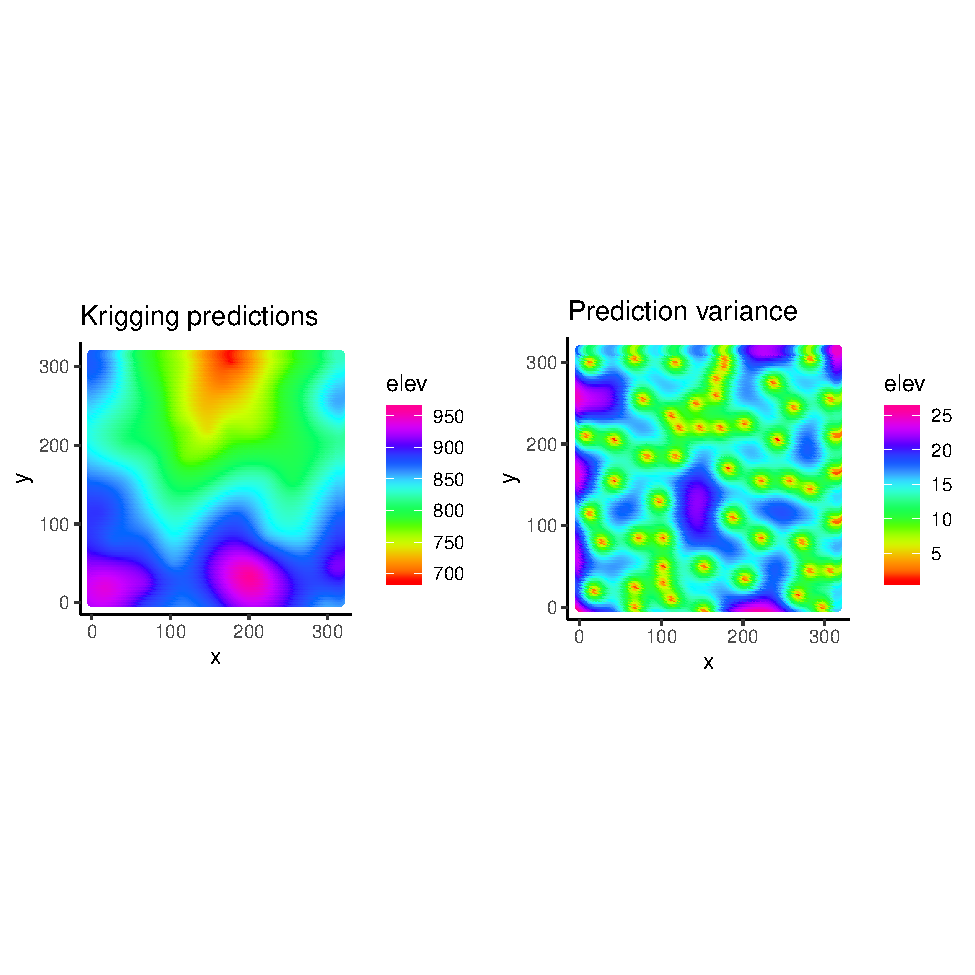
\includegraphics{Exercise-1_files/figure-latex/fig3-1.pdf}
\caption{\label{fig:fig3} Krigging predictions and prediction variance
of the ordinary krigging method.}
\end{figure}

\hypertarget{problem-2d}{%
\subsection{Problem 2d}\label{problem-2d}}

The resulting polynomial function becomes: \[
\vect{(gx)} = (1, x_v, x_h, x_vx_h, x_v^2, x_h^2)
\] The expected value of \(r(\vect{x})\) then is: \[
E \{r(\vect{x}) \} = \beta_1 + \beta_2x_v + \beta_3x_h + \beta_4x_vx_h + \beta_5x_v^2 + \beta_6x_h^2 .
\]

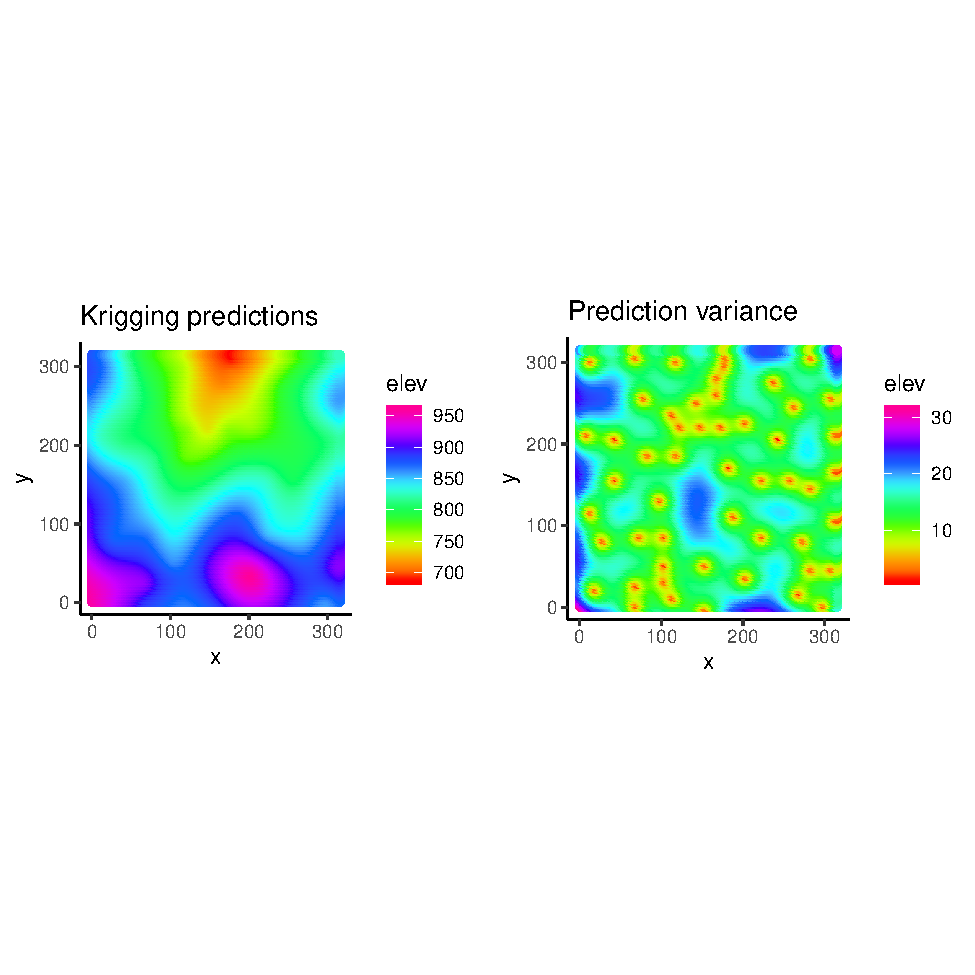
\includegraphics{Exercise-1_files/figure-latex/fig4-1.pdf} We present
the predictions and the associated variance in Figure \ref{fig:fig4}

\hypertarget{problem-2e}{%
\subsection{Problem 2e}\label{problem-2e}}

We now consider the grid node, \(\vect{x_0} = (100,100)\). Using the
ordinary krigging, we estimated the predicted mean as 838.6781414 and
the predicted variance as 10.044233. Assuming Gaussianity of the data,

\begin{equation*}
    \begin{split}
P(r\{\vect{x_0}\} > 850) &=P\bigg( \frac{r\{\vect{x_0}\}- E(r\{\vect{x_0}\})}{\sqrt{Var(r\{\vect{x_0}\})}}> \frac{850- E(r\{\vect{x_0}\})}{\sqrt{Var(r\{\vect{x_0}\})}} \bigg)\\
&= 1 - \Phi\bigg(\frac{850- E(r\{\vect{x_0}\})}{\sqrt{Var(r\{\vect{x_0}\})}} \bigg)
  \end{split}
\end{equation*}

The resulting probability is 0.13.

To obtain the elevation for which it is 0.90 probability that the true
elevation is below it, we used the formular,

\begin{equation*}
    \begin{split}    
P(r\{\vect{x_0}\} >r\{\vect{x_{new}}\} ) &= 0.90\\
r\{\vect{x_{new}}\} &= E(r\{\vect{x_0}\}) + \phi(0.90) \sqrt{Var(r\{\vect{x_0}\})}
  \end{split}
\end{equation*}

We obatained 851.55m to be that elevation that satifies the preamble.

\newpage

\hypertarget{problem-3}{%
\section{Problem 3}\label{problem-3}}

We consider the stationary Gaussian RF
\(\lbrace r((\vect x); \vect x \in D \subset \mathbb{R}^2\). With
\(D:\left[(1,30) \times (1,30) \right]\).

With: \begin{equation}
    \begin{split}
        E\lbrace r(\vect x) \rbrace &= \mu_r = 0 \\
        Var\lbrace r(\vect x) \rbrace &= \sigma_r^2 \\
        Corr\lbrace r(\vect x), r(\vect x')\rbrace \\
        &= exp\lbrace -\frac{\tau}{\xi_r}\rbrace
    \end{split}
\end{equation}

with \(\tau = |\vect x - \vect x'|\)

\hypertarget{problem-3ac}{%
\subsection{Problem 3ac}\label{problem-3ac}}

Discretize the random field with
\(L:\left[(1,30) \times (1,30)\right] \in D\) with parameters
\(\sigma_r^2\) and \(\xi_r = 3\). And simulate realizations.

\begin{figure}

{\centering 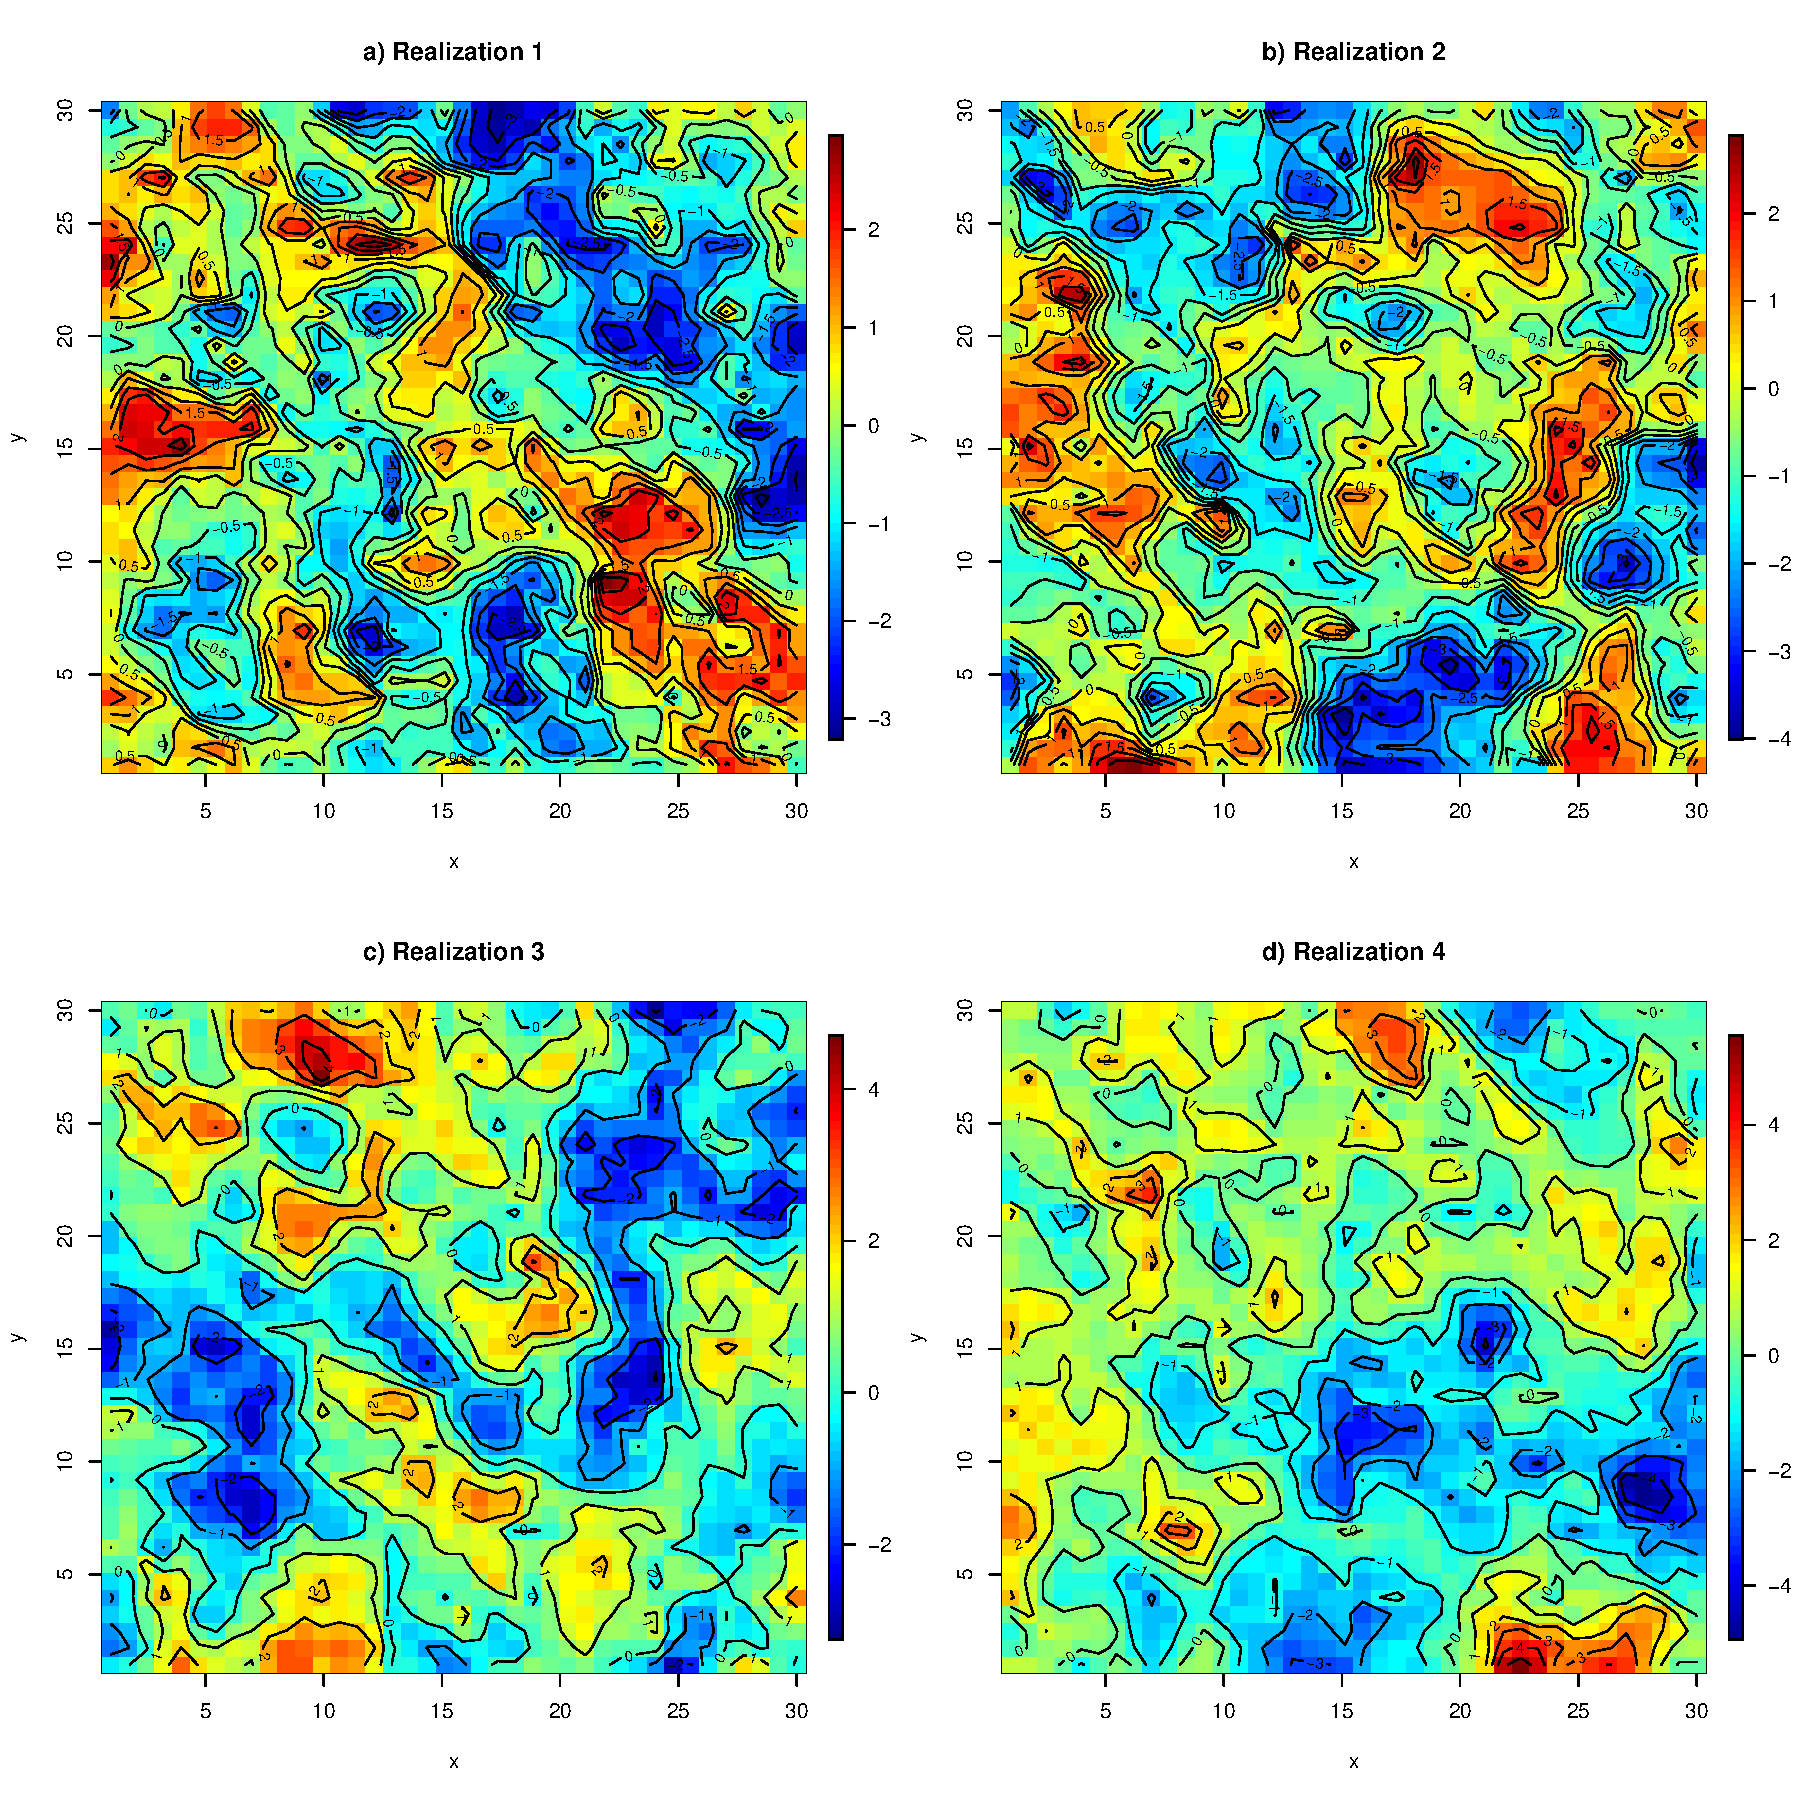
\includegraphics{Exercise-1_files/figure-latex/fig3a1-1} 

}

\caption{\label{fig:fig3a1} Realizations of field with $\xi = 3$, $\sigma^2 = 2$}\label{fig:fig3a1}
\end{figure}

Create four realizations that are presented in Figure \ref{fig:fig3a1}

\hypertarget{problem-3bc}{%
\subsection{Problem 3bc}\label{problem-3bc}}

The theoretical variogram function can be written as: \begin{equation}
    \gamma_r(\tau) =  \sigma_r^2(1-\rho_r(\tau))
\end{equation}

We plot the emprical variogram from our realisations and compare to the
theoretical variogram.

\begin{figure}

{\centering 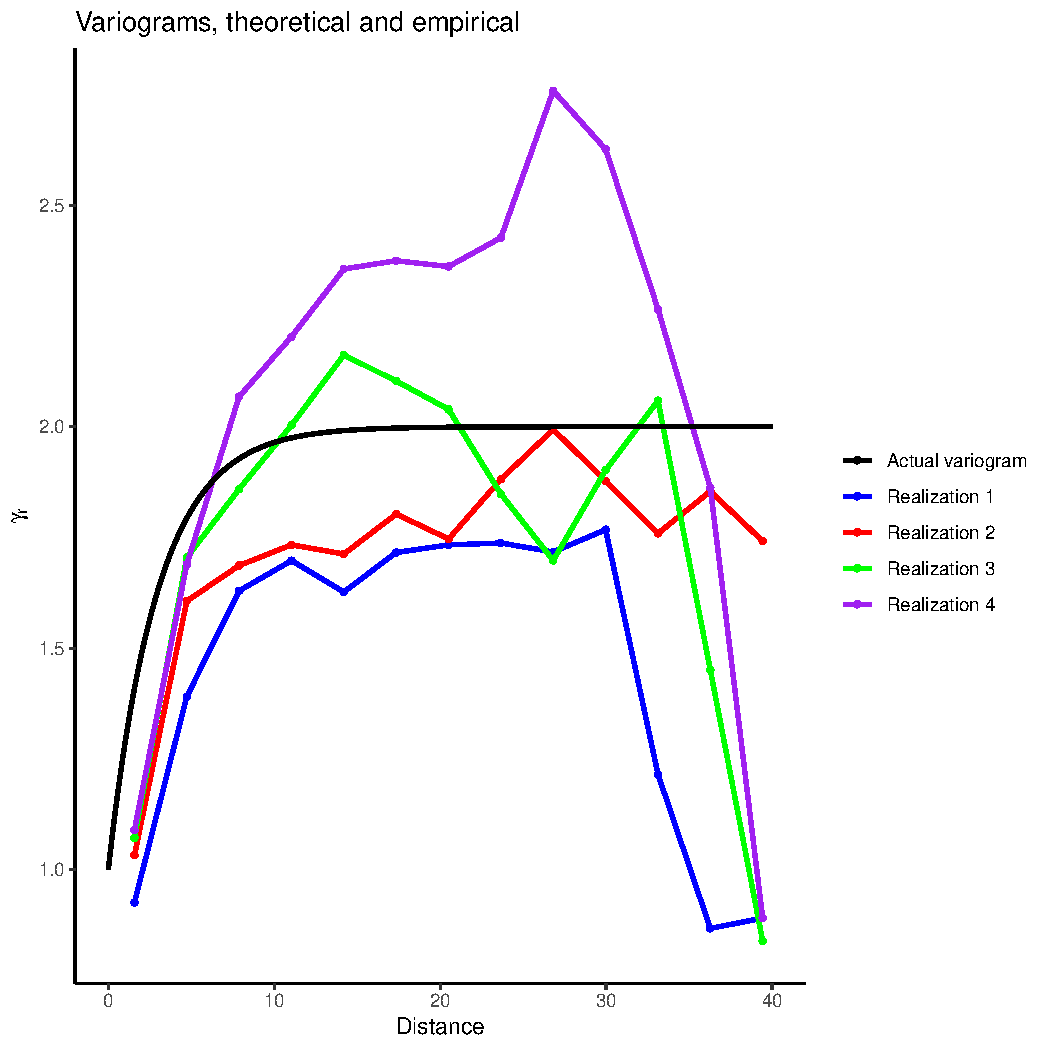
\includegraphics{Exercise-1_files/figure-latex/fig3b1-1} 

}

\caption{\label{fig:fig3b1} Empirical variogram vs. theoretical variogram of realisation in Figure \ref{fig:fig3a1}.$\xi = 3$, $\sigma^2 = 2$}\label{fig:fig3b1}
\end{figure}

The results are plotted in Figure \ref{fig:fig3b1}. None of the
empirical variograms seem to be very accurate. The seem to capture the
shape of the theoretical variogram at low distances, however at large
distances the empirical variograms vary alot, this is probably due to a
low amount of points that have a large distance in between.

\newpage

\hypertarget{problem-3de}{%
\subsection{Problem 3de}\label{problem-3de}}

Generate 36 point uniformly on \(L\). And simulate a realisation over
those 36 points. Will later take on these as exact observations.

Use \textbf{likfit} to estimate the parameters of our field using our 36
exact observations.

The summary of the \textbf{likfit} is displayed inbelow:

\begin{Shaded}
\begin{Highlighting}[]
\KeywordTok{summary}\NormalTok{(likfit}\FloatTok{.36}\NormalTok{)}
\end{Highlighting}
\end{Shaded}

\begin{verbatim}
## Summary of the parameter estimation
## -----------------------------------
## Estimation method: maximum likelihood 
## 
## Parameters of the mean component (trend):
##   beta 
## 0.8442 
## 
## Parameters of the spatial component:
##    correlation function: exponential
##       (estimated) variance parameter sigmasq (partial sill) =  2.255
##       (estimated) cor. fct. parameter phi (range parameter)  =  1.869
##    anisotropy parameters:
##       (fixed) anisotropy angle = 0  ( 0 degrees )
##       (fixed) anisotropy ratio = 1
## 
## Parameter of the error component:
##       (estimated) nugget =  0
## 
## Transformation parameter:
##       (fixed) Box-Cox parameter = 1 (no transformation)
## 
## Practical Range with cor=0.05 for asymptotic range: 5.599689
## 
## Maximised Likelihood:
##    log.L n.params      AIC      BIC 
## "-64.19"      "4"  "136.4"  "142.7" 
## 
## non spatial model:
##    log.L n.params      AIC      BIC 
## "-67.12"      "2"  "138.2"  "141.4" 
## 
## Call:
## likfit(geodata = geo, ini.cov.pars = c(1, 1), cov.model = "exponential")
\end{verbatim}

Using the 36 point we estimate \(\hat\sigma^2 =\) 2.254746 and
\(\hat \xi =\) 1.8692279. We repeat the process in 3d for \(n=6\),
\(n=64\), \(n=100\).

\newpage

The ML estimates of the parameters were:

\begin{longtable}[]{@{}lll@{}}
\toprule
n & \(\hat \sigma^2_{ML}\) & \(\hat\xi_{ML}\)\tabularnewline
\midrule
\endhead
9 & 1.1269907 & 0.28203\tabularnewline
36 & 2.254746 & 1.8692279\tabularnewline
64 & 2.4823404 & 4.7979249\tabularnewline
100 & 2.1700308 & 3.3909212\tabularnewline
-------- & ----------------------- & -------------------\tabularnewline
Actual & 2 & 3\tabularnewline
\bottomrule
\end{longtable}

We see that the estimates becomes quite accurate at large values of
\(n\), and be very off at lower values of \(n\)

We plot the empirical variograms vs theoretical.

\begin{figure}
\centering
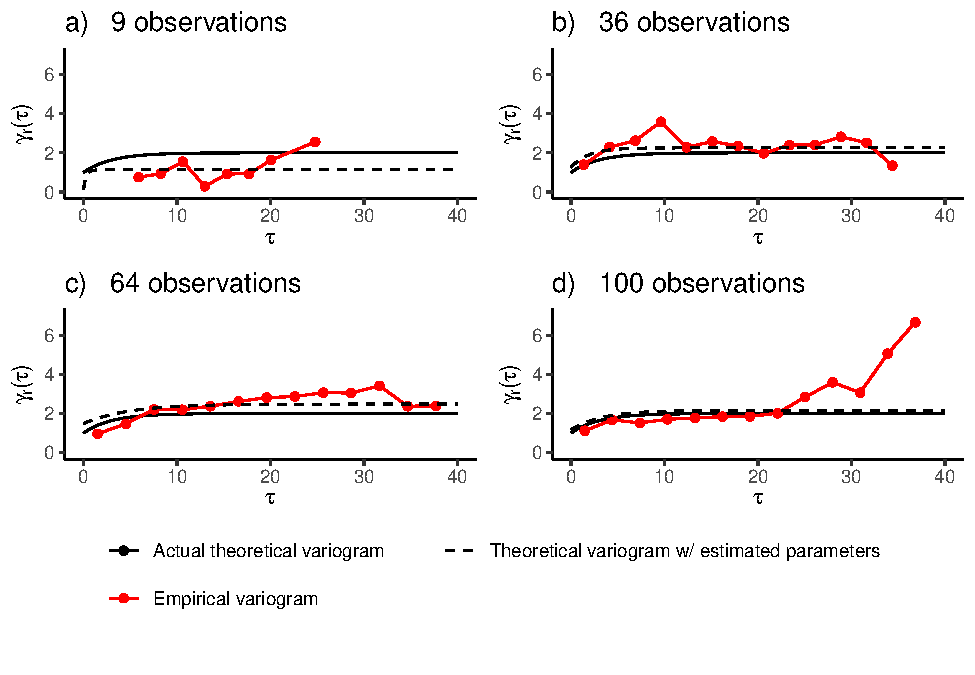
\includegraphics{Exercise-1_files/figure-latex/unnamed-chunk-8-1.pdf}
\caption{\label{fig:fig3d2} Variograms from uniform drawn points
\(\xi = 3\), \(\sigma^2 = 2\), maximum likelihood fit}
\end{figure}

These variograms are displayed in Figure \ref{fig:fig3d2}. They seem to
vary quite much, but that can probably be blamed on a low amount of
observation points. As we draw a very limited amount of points, some
distances will be less represented than others, which will cause large
variations in estimation. This can especially be seen for \(n=9\).

\hypertarget{problem-3f}{%
\section{Problem 3f}\label{problem-3f}}

In this problem we have used maxmium likelihood to estiamte the
parameters of the correlation funciton. We have found that using maximum
likelihood to estiamte parameters seems to be relatively fast using the
number of parameters and observations we have here (although
\textbf{likfit} warns that the opposite might be the case). With enough
data points maximum likelihood seems to be quite good at finding the
correct parameters.


\end{document}
